\begin{frame}{Annexe}{Le cadre $\mathcal{M}OISE^+$ (2/2)}

    \vspace{-2.5ex}

    \begin{columns}
        \hspace{-16ex}
        \begin{column}{0.5\textwidth}
            \centering
            \begin{figure}[H]
                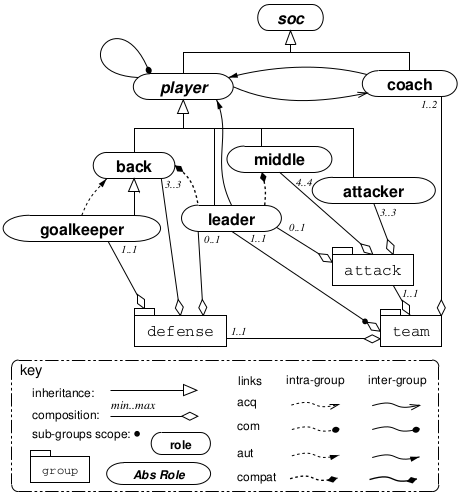
\includegraphics[width=0.7\textwidth]{figures/soccer_ss.png}
                \caption*{Spécifications structurelles}
            \end{figure}
        \end{column}
        \hspace{-20ex}
        \begin{column}{0.5\textwidth}
            \centering
            \begin{figure}[H]
                \centering
                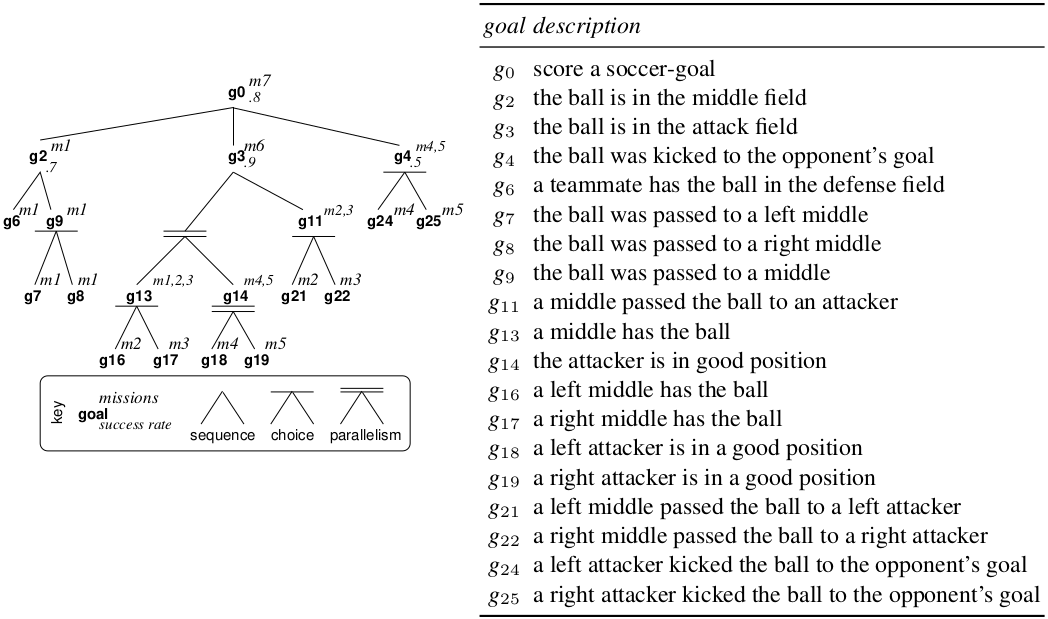
\includegraphics[width=1.2\textwidth]{figures/soccer_fs.png}
                \caption*{Spécifications fonctionnelles}
            \end{figure}
        \end{column}
    \end{columns}

    \ \\

    \begin{minipage}{\textwidth}
        \centering
        \begin{figure}[H]
            \centering
            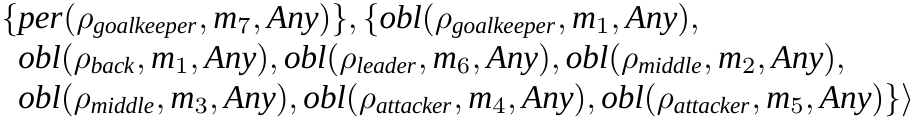
\includegraphics[width=0.4\linewidth]{figures/soccer_ds.png}
            \caption*{Spécifications déontiques}
        \end{figure}
    \end{minipage}

\end{frame}

\begin{frame}{Annexe}{Q : Les contraintes organisationnelles nuisent-elles à l'exploration ?}
    \begin{itemize}
        \item \textbf{Pas nécessairement.} Les contraintes peuvent en réalité \textit{guider l'exploration} de manière plus efficace en élaguant les comportements non prometteurs.
        \item La dureté de contrainte (hardness) permet d’ajuster la rigueur avec laquelle les agents suivent les rôles/objectifs.
        \item Avec des contraintes souples, les agents conservent leur capacité d'exploration tout en étant orientés vers des comportements structurés.
    \end{itemize}
\end{frame}

\begin{frame}{Annexe}{Q : En quoi MOISE+MARL est-il différent du RL hiérarchique ?}
    \begin{itemize}
        \item Le RL hiérarchique décompose les tâches de manière interne via des hiérarchies apprises.
        \item MOISE+MARL impose des \textbf{rôles et missions organisationnels externes} comme contraintes comportementales.
        \item Les rôles sont \textit{interprétables, configurables et découplés de l’architecture de l’agent}.
    \end{itemize}
\end{frame}

\begin{frame}{Annexe}{Q : Votre cadre passe-t-il à l’échelle avec de nombreux agents ? Et la plasticité des politiques ?}
    \begin{itemize}
        \item Scalabilité : les rôles peuvent être \textbf{abstraits} et appliqués à des groupes d’agents (ex. “défenseur”, “collecteur”).
        \item Plasticité : la dureté des contraintes est ajustable. Les contraintes souples préservent l’adaptabilité des politiques.
        \item Compromis : des contraintes fortes apportent de la stabilité, les contraintes souples offrent de la flexibilité.
    \end{itemize}
\end{frame}

\begin{frame}{Annexe}{Q : Comment MOISE+MARL gère-t-il la partialité d’observation ?}
    \begin{itemize}
        \item Basé sur le formalisme Dec-POMDP : la partialité d’observation est gérée nativement.
        \item Les contraintes s’appliquent aux \textbf{trajectoires observées} des agents — et non aux états globaux.
        \item Aucun besoin de connaissance globale ou de contrôle centralisé.
    \end{itemize}
\end{frame}

\begin{frame}{Annexe}{Q : La méthode TEMM est-elle coûteuse ? Peut-elle généraliser ?}
    \begin{itemize}
        \item TEMM est appliquée après l'entraînement. Elle utilise du clustering (K-means, hiérarchique) et peut être parallélisée.
        \item Elle s’applique à tout environnement avec des trajectoires étiquetées, et ne dépend pas de l’algorithme d’apprentissage.
        \item Actuellement hors-ligne uniquement ; des extensions temps réel sont à l’étude.
    \end{itemize}
\end{frame}

\begin{frame}{Annexe}{Q : Comment évaluez-vous l’impact des contraintes organisationnelles ?}
    \begin{itemize}
        \item Nous comparons une référence de base (sans contraintes) à une base contrainte (MOISE+MARL).
        \item Métriques : Récompense Cumulative, Taux de Convergence, Ajustement Organisationnel, Cohérence, Robustesse, Taux de Violation.
        \item MOISE+MARL améliore systématiquement l’ajustement organisationnel et la stabilité dans tous les environnements testés.
    \end{itemize}
\end{frame}

% ===============
\begin{frame}{Annexe}
    {Contexte}

    \begin{block}{Paradigme des Systèmes Multi-Agents (SMA) pour des problèmes complexes et distribués}
        \begin{itemize}
            \item \textbf{décomposition de tâches} : missions déléguées, coopération~\parencite{Raileanu2023} ;
            \item \textbf{avantages} : gestion d’objectifs, calcul parallèle, robustesse, passage à l’échelle\dots
        \end{itemize}
    \end{block}

    \begin{block}{\textbf{Organisation} : élément clé dans la conception des SMA}
        \begin{itemize}
            \item \textbf{coordination} : atteindre objectif collaborativement~\parencite{Hubner2007} ;
            \item \textbf{environnements dynamiques et incertains} : flexibilité, adaptation~\parencite{Kathleen2020} ;
        \end{itemize}
    \end{block}

    \begin{block}{Méthodes et pratiques pour la conception de SMA}
        \begin{itemize}
            \item \textbf{approche + modèle organisationnel} : méthodes reposent sur expérience des concepteurs pour créer manuellement \textbf{politiques} afin que le SMA atteigne ses objectifs ;
            \item \textbf{de la simulation à la réalité} : 1) conception sûre et efficace dans un environnement simulé fidèle ; \quad 2) transfert vers l’environnement réel~\parencite{Schon2021}.
        \end{itemize}
        \quad $\Longrightarrow$ \textbf{Processus itératif basé sur essais et erreurs}
    \end{block}

\end{frame}

\begin{frame}{Annexe}{CAGE Challenge 3}
    \begin{figure}
        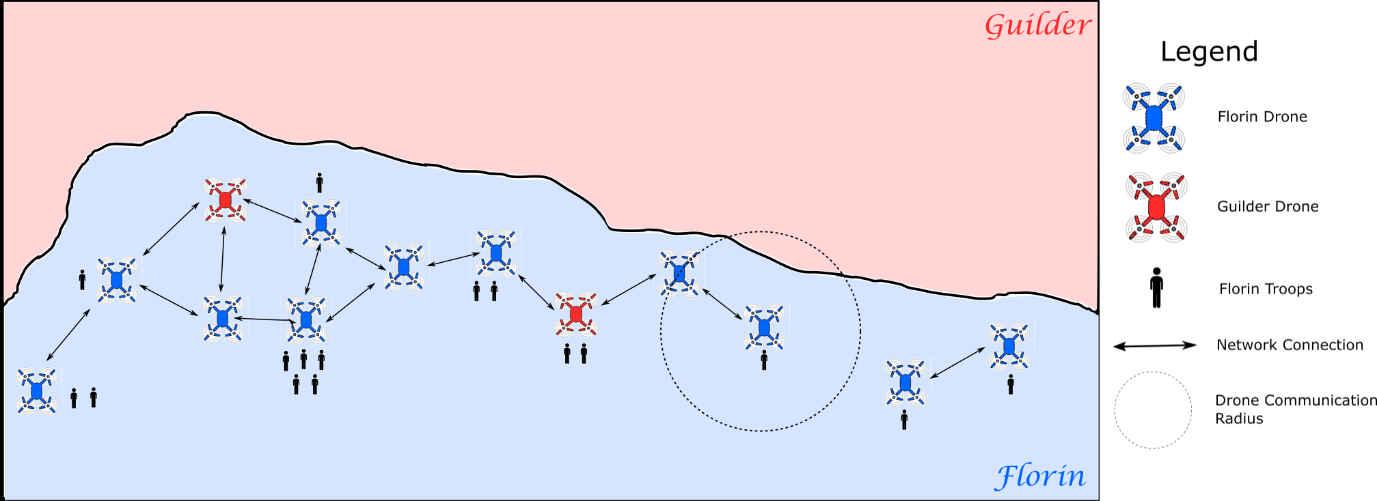
\includegraphics[width=0.9\linewidth]{figures/cage_challenge_3.png}
        \caption*{Les forces de Florin patrouillent à la frontière avec Guilder, en utilisant un réseau ad hoc fourni par des drones aériens. Ici, Guilder a réussi à corrompre deux drones de ce réseau et peut ainsi intercepter ou modifier une partie des messages échangés.}
    \end{figure}
\end{frame}

\begin{frame}{Annexe}{Prédateur-proie}
    \begin{figure}
        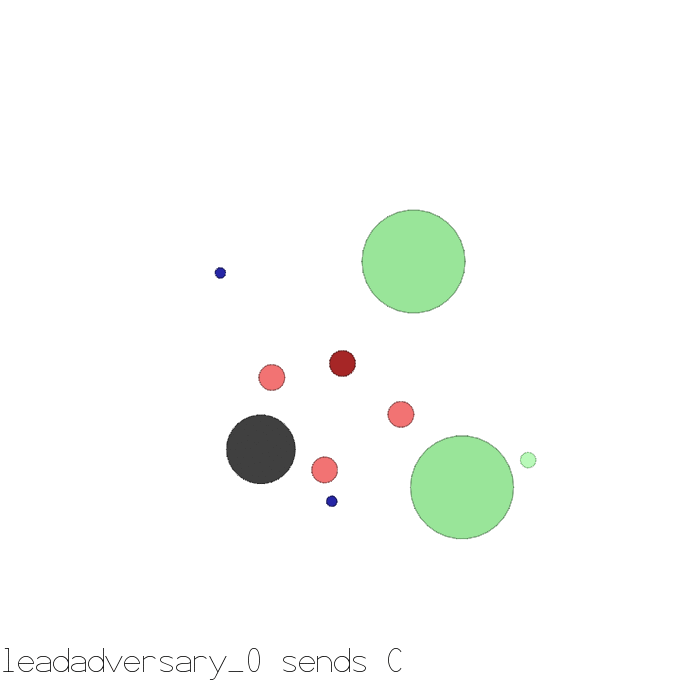
\includegraphics[width=0.5\linewidth]{figures/mpe_simple_world_comm.png}
    \end{figure}
\end{frame}

\begin{frame}{Annexe}
    {Notions de base sur les SMA}

    \begin{block}{Mots-clés}
        \begin{itemize}
            \item \textbf{Agent} : entité immergée dans un environnement, percevant des observations et prenant des décisions de manière autonome pour atteindre des objectifs ;
            \item \textbf{SMA} : ensemble d’agents collaborant avec des mécanismes d’auto-(ré)organisation pour atteindre leurs objectifs ;
            \item \textbf{Organisation} : interactions entre agents, explicites ou implicites ;
            \item \textbf{Modèle Organisationnel (MO)} : support pour décrire formellement une organisation explicite ou implicite ;
            \item \textbf{Spécifications Organisationnelles (OS)} : composants d’un MO servant à caractériser une organisation.
        \end{itemize}
    \end{block}

    \begin{block}{Modèle organisationnel : $\mathcal{M}OISE^+$}
        \begin{itemize}
            \item plus complexe que \emph{Agent Group Roles} (intégration de standards) ;
            \item prend explicitement en compte les aspects sociaux entre agents ;
            \item permet de relier les politiques des agents aux spécifications organisationnelles.
        \end{itemize}
    \end{block}

\end{frame}
\begin{frame}{Annexe}
    {Notions de base en MARL}

    \begin{block}{Mots-clés}
        \begin{itemize}
            \item \textbf{Politique} : la « logique » utilisée par un agent pour choisir la prochaine action en fonction de son observation ;
            \item \textbf{Historique/trajectoire} : la suite des couples (observation, action) au cours d’un épisode ;
            \item \textbf{Politique conjointe / Historique conjoint} : l’ensemble des politiques / historiques de tous les agents ;
            \item \textbf{Apprentissage par renforcement} : un agent met à jour sa politique pour maximiser une récompense cumulative ;
            \item \textbf{Apprentissage par renforcement multi-agent (MARL)} : extension à plusieurs agents apprenant en tenant compte des actions des autres.
        \end{itemize}
    \end{block}

\end{frame}

\begin{frame}{Annexe}{Méthode MAMAD : Vue d’ensemble}

    \begin{columns}

        \begin{column}{0.6\textwidth}

            \textbf{Phase 1 : Modélisation}

            \begin{itemize}
                \item Développer manuellement un environnement simulé ($1.1$) dans lequel les agents doivent coopérer pour atteindre un objectif ($1.2$) ;
                \item Possibilité de définir les comportements attendus des rôles comme des historiques ;
                \item Possibilité de contraindre les agents à certains rôles ($1.3$).
            \end{itemize}

        \end{column}

        \begin{column}{0.4\textwidth}
            \centering
            \adjustbox{trim={0.\width} {0.82\height} {0.\width} {0.\height}, clip}{%
                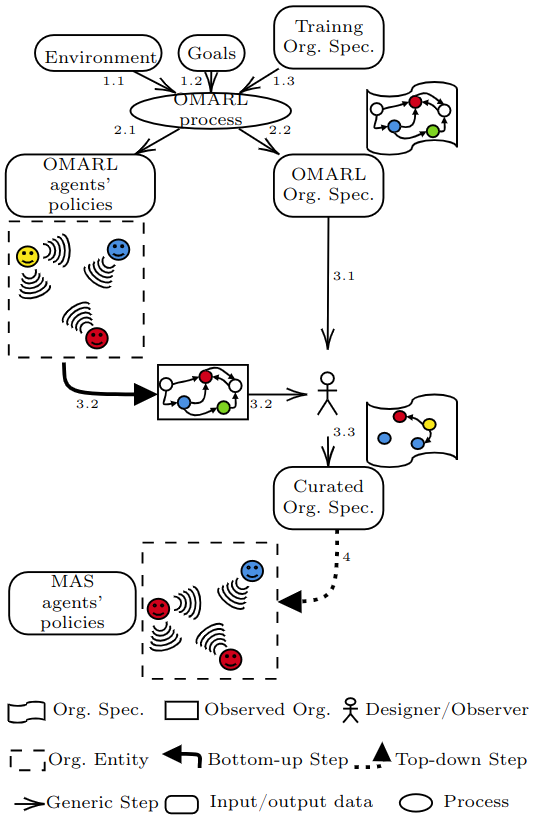
\includegraphics[width=1.2\linewidth]{figures/AOMEA_illustrative_view}
            }
        \end{column}

    \end{columns}

\end{frame}


\begin{frame}{Annexe}{Méthode MAMAD : Vue d’ensemble}

    \begin{columns}

        \begin{column}{0.6\textwidth}

            \textbf{Phase 2 : Résolution}

            \begin{itemize}
                \item Algorithme OMARL (Organisation-oriented MARL) : processus MARL enrichi par un modèle organisationnel ;
                \item Apprentissage visant à satisfaire les historiques contraints des rôles ($2.1$) ;
                \item Obtention de spécifications organisationnelles associées ($2.2$).
            \end{itemize}

        \end{column}

        \begin{column}{0.4\textwidth}
            \centering
            \adjustbox{trim={0.\width} {0.56\height} {0.\width} {0.\height}, clip}{%
                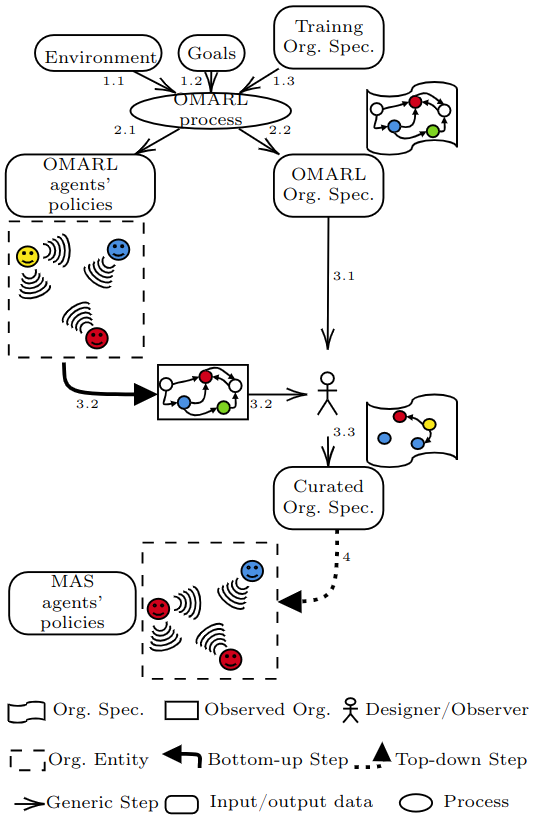
\includegraphics[width=1.2\linewidth]{figures/AOMEA_illustrative_view}
            }
        \end{column}

    \end{columns}

\end{frame}

\begin{frame}{Annexe}{Méthode MAMAD : Vue d’ensemble}

    \begin{columns}

        \begin{column}{0.6\textwidth}

            \textbf{Phase 3 : Analyse}

            \begin{itemize}
                \item Les concepteurs observent les politiques apprises des agents ($3.2$) ;
                \item Ils examinent les spécifications organisationnelles calculées ($3.1$) pour comprendre comment les agents atteignent l’objectif ;
                \item Ils obtiennent des indications pour concevoir un SMA opérationnel : spécifications organisationnelles sélectionnées ($3.3$).
            \end{itemize}

        \end{column}

        \begin{column}{0.4\textwidth}
            \centering
            \adjustbox{trim={0.\width} {0.35\height} {0.\width} {0.188\height}, clip}{%
                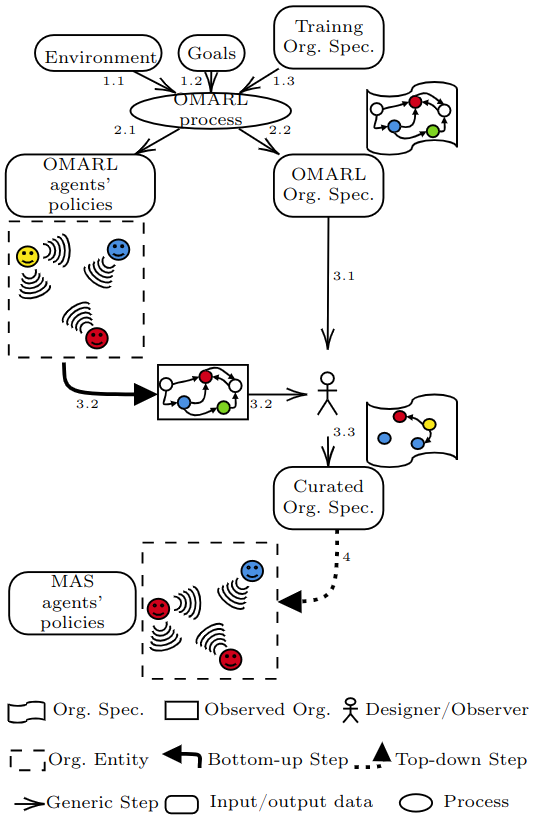
\includegraphics[width=1.2\linewidth]{figures/AOMEA_illustrative_view}
            }
        \end{column}

    \end{columns}

\end{frame}

\begin{frame}{Annexe}{Méthode MAMAD : Vue d’ensemble}

    \begin{columns}

        \begin{column}{0.6\textwidth}

            \textbf{Phase 4 : Déploiement / Développement}

            \begin{itemize}
                \item Les concepteurs utilisent les spécifications sélectionnées pour implémenter un SMA ;
                \item Développement d’un SMA classique avec prise en compte des questions de sûreté ;
                \item Le SMA est évalué par simulation.
            \end{itemize}

        \end{column}

        \begin{column}{0.4\textwidth}
            \centering
            \adjustbox{trim={0.\width} {0.15\height} {0.\width} {0.57\height}, clip}{%
                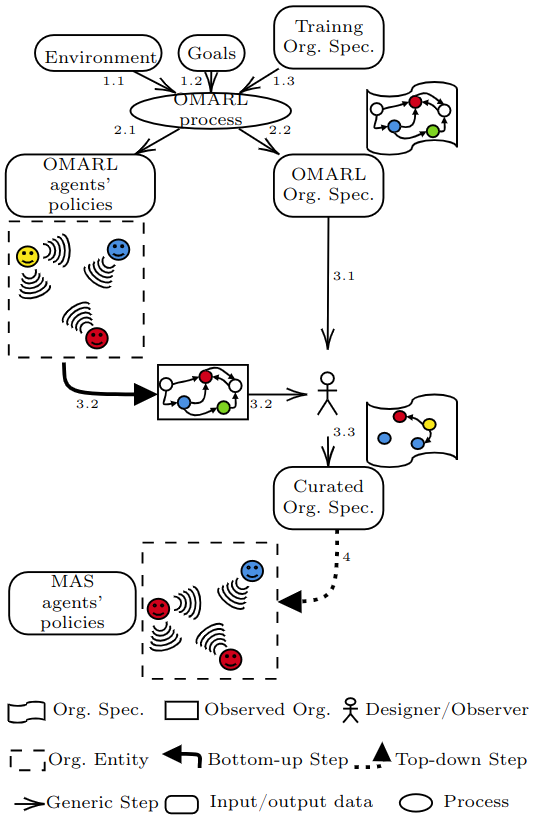
\includegraphics[width=1.2\linewidth]{figures/AOMEA_illustrative_view}
            }
        \end{column}

    \end{columns}

\end{frame}


\begin{frame}{Appendix}{Trajectory-based Evaluation in MOISE+MARL}

    \textbf{Inferring Organizational Specifications}

    \begin{columns}

        \begin{column}{0.3\textwidth}

            \begin{itemize}
                \item \textbf{Knowledge-based Organizational Specifications Identification (KOSIA)}
                \item \textbf{General Organizational Specifications Infererence (GOSIA)}
            \end{itemize}

        \end{column}

        \begin{column}{0.8\textwidth}
            \begin{figure}
                \centering
                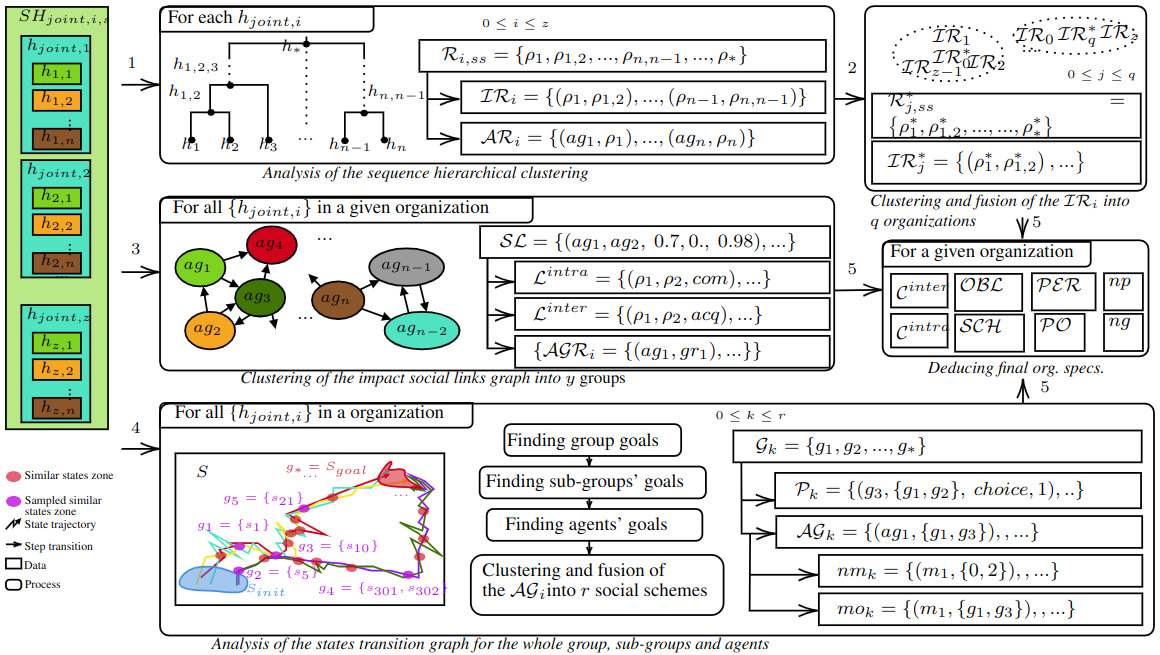
\includegraphics[width=0.95\linewidth]{figures/GOSIA_view.png}
                \caption*{A summary view of the GOSIA process}
                \label{fig:gosia_process}
            \end{figure}
        \end{column}

    \end{columns}

\end{frame}
\begin{frame}{Annexe}{Apprentissage par renforcement contraint (Constrained-RL)}

    \begin{itemize}
        \item Apprendre une politique qui maximise la récompense tout en respectant des contraintes de \textbf{sûreté} ou de \textbf{performance}.

        \item \textbf{Contraintes dures} : doivent être toujours respectées (ex. : \textit{Shielding}).
        \item \textbf{Contraintes souples} : respectées en moyenne ou via des pénalités.

        \item \textbf{Principales méthodes :}
              \begin{itemize}
                  \item \textbf{Modelage de récompense (Reward Shaping)} : ajouter des pénalités lorsque les contraintes sont violées.
                  \item \textbf{Projection de politique} : ajuster les actions pour rester dans les limites.
                  \item \textbf{Variables duales} : utiliser des multiplicateurs de Lagrange pour gérer les contraintes.
              \end{itemize}
    \end{itemize}

\end{frame}

\begin{frame}{Annexe}{\textit{Safe exploration} et \textit{Shielding} en apprentissage par renforcement}

    \begin{itemize}
        \item \textbf{\textit{Safe exploration}} $\rightarrow$ garantir la sûreté pendant l'exploration en limitant les comportements risqués.
        \item Principalement en modifiant la fonction de récompense (ex. : via Lagrangiens)
        \item \textbf{\textit{Shielding}} : intervenir en temps réel pour bloquer les actions dangereuses et garantir une \textit{Safe exploration}.
    \end{itemize}

    \textbf{Référence :} \\
    \textit{Akifumi Wachi, Wataru Hashimoto, Xun Shen, \& Kazumune Hashimoto (2023). Safe Exploration in Reinforcement Learning: A Generalized Formulation and Algorithms. In NeurIPS 2023.}

\end{frame}

\begin{frame}[fragile]{Annexe}{Exemple d’utilisation d’Optuna}
    \begin{itemize}
        \item \textbf{Optuna} est une bibliothèque open-source pour l’optimisation des hyperparamètres (HPO), largement utilisée en apprentissage automatique.
        \item Exemples d’hyperparamètres : taux d’apprentissage, fonction d’activation, nombre de couches, taille des couches, seuil de distance pour le clustering, etc.
        \item \textbf{Étapes pour utiliser Optuna :}
              \begin{itemize}
                  \item \texttt{1.} Définir une fonction objectif.
                  \item \texttt{2.} Lancer une étude avec Optuna.
                  \item \texttt{3.} Utiliser le meilleur résultat pour entraîner le modèle.
              \end{itemize}
    \end{itemize}

    \begin{lstlisting}[language=Python, basicstyle=\small\ttfamily, frame=single, caption=Exemple d'utilisation d'Optuna en Python]
import optuna

def objective(trial):
    x = trial.suggest_float("x", -10, 10)
    return (x - 2) ** 2  # Fonction fictive

study = optuna.create_study(direction="minimize")
study.optimize(objective, n_trials=100)

print(study.best_params)  # Affiche les meilleurs parametres
    \end{lstlisting}
\end{frame}

\begin{frame}{Annexe}{Présentation de PettingZoo}

    \begin{itemize}
        \item Bibliothèque Python pour les environnements multi-agents.
        \item Facilite l'entraînement et l'évaluation d'agents dans différents contextes multi-agents.

        \item \textbf{Fonctionnalités principales :}
              \begin{itemize}
                  \item Prise en charge de différents types d’environnements (tour par tour, parallèle, etc.).
                  \item Intégration facile avec des frameworks RL comme RLlib.
                  \item Compatible avec les API Gym pour une utilisation intuitive.
              \end{itemize}

        \item \textbf{Exemples d’environnements inclus :}
              \begin{itemize}
                  \item Jeux : \textit{TicTacToe}, \textit{ConnectFour}
                  \item Collaboration/compétition : \textit{Pistonball}, \textit{Dilemme du prisonnier}
                  \item Intégration avec la suite Atari multi-agents
              \end{itemize}
    \end{itemize}

\end{frame}

\begin{frame}[fragile]{Annexe}{Exemple d'utilisation de PettingZoo}
    \begin{itemize}
        \item Exemple : créer et interagir avec un environnement.
        \item Charger l’environnement, le réinitialiser, puis interagir étape par étape avec les agents.
    \end{itemize}
    \vspace{0.3cm}
    \begin{lstlisting}[language=Python, basicstyle=\ttfamily\small]
from pettingzoo.butterfly import pistonball_v6

# Creation et reinitialisation de l environnement
env = pistonball_v6.env()
env.reset()

# Boucle d interaction
for agent in env.agent_iter():
    obs, reward, done, info = env.last()
    action = env.action_space(agent).sample()  # Action aleatoire
    env.step(action)
    if done:
        env.reset()  # Reinitialisation si episode termine
    \end{lstlisting}
\end{frame}

\begin{frame}{Annexe}{KB-Org}
    \frametitle{Systèmes multi-agents basés sur l'organisation : de la modélisation à l'implémentation}

    \begin{itemize}
        \item Modélise et implémente des SMA basés sur une organisation explicite ;
        \item Intègre des concepts organisationnels pour structurer les comportements et interactions ;
        \item Fournit un référentiel de modèles organisationnels prêts à l'emploi ;
        \item Vise à améliorer l'explicabilité et la coordination.
    \end{itemize}

    \vspace{1em}
    Sims, V. (2008). Automated organization design for multi-agent systems. Autonomous Agents and Multi-Agent Systems, 16(2), 151–185.

\end{frame}

\begin{frame}{Annexe}{Présentation de MARLlib}

    \begin{itemize}
        \item Bibliothèque Python pour l’apprentissage par renforcement multi-agent (MARL) ;
        \item Supporte plusieurs environnements : PettingZoo, StarCraft II, MPE, etc. ;
        \item Implémente plusieurs algorithmes MARL : MADDPG, MAPPO, etc. ;
        \item Propose des outils pour l'entraînement, l’évaluation et la comparaison d’algorithmes ;
        \item Fournit des configurations prêtes à l’emploi ajustées pour divers environnements.
    \end{itemize}

\end{frame}

\begin{frame}[allowframebreaks]{Annexe}{Aperçu des algorithmes dans MARLlib}

    \begin{itemize}
        \item \textbf{Algorithmes basés sur la valeur}
              \begin{itemize}
                  \item \textbf{Multi-Agent Q-Learning} : Extension multi-agent de Q-learning.\newline
                        \textit{Remarque : simple mais souffre de problèmes d’échelle et de non-stationnarité.}
                  \item \textbf{MADDPG} : Extension de DDPG au cadre multi-agent.\newline
                        \textit{Remarque : adapté aux actions continues mais gourmand en données et complexe.}
              \end{itemize}

        \item \textbf{Algorithmes basés sur la politique}
              \begin{itemize}
                  \item \textbf{REINFORCE} : Méthode de gradient de politique basique.\newline
                        \textit{Remarque : fonctionne en environnements stochastiques, mais variance élevée.}
                  \item \textbf{MAPPO (Multi-Agent PPO)} : Extension multi-agent de PPO.\newline
                        \textit{Remarque : stabilise les mises à jour, mais nécessite du réglage et des ressources.}
              \end{itemize}

        \item \textbf{Algorithmes hybrides}
              \begin{itemize}
                  \item \textbf{A3C} : Combine apprentissage de la valeur et de la politique.\newline
                        \textit{Remarque : apprentissage rapide mais synchronisation complexe.}
                  \item \textbf{MAPPO} : Variante hybride basée sur PPO avec entraînement centralisé.\newline
                        \textit{Remarque : efficace pour les tâches coopératives, mais coûteux.}
              \end{itemize}

        \item \textbf{Algorithmes théoriques ou basés sur la théorie des jeux}
              \begin{itemize}
                  \item \textbf{IQL (Independent Q-Learning)} : Q-learning par agent, sans coordination.\newline
                        \textit{Remarque : simple à implémenter, mais souffre de non-stationnarité.}
                  \item \textbf{COMA} : Utilise des contre-factuels pour évaluer la contribution des agents.\newline
                        \textit{Remarque : réduit la variance, améliore la coopération, mais coûteux.}
              \end{itemize}

        \item \textbf{Entraînement centralisé avec exécution décentralisée (CTDE)}
              \begin{itemize}
                  \item \textbf{QMIX} : Décompose les Q-valeurs pour permettre la coordination.\newline
                        \textit{Remarque : bon compromis entre apprentissage centralisé et exécution décentralisée.}
                  \item \textbf{VDN (Value Decomposition Networks)} : Coordination par décomposition des valeurs.\newline
                        \textit{Remarque : efficace, mais limité pour les interactions complexes.}
              \end{itemize}
    \end{itemize}

\end{frame}
